\section{Příklad 2}
% Jako parametr zadejte skupinu (A-H)
\druhyZadani{G}

\subsection{Krok 1}
Najskor musime nahradit zdroj U za skrat a namiesto rezistoru $R_3$ dat roztvorene svorky.

\begin{figure}[!h]
    \centering
    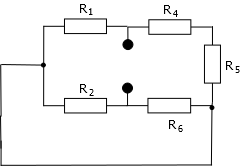
\includegraphics[width=0.5\linewidth]{pr2/1.png}
\end{figure}

\subsection{Krok 2}
Obvod preusporiadame a zistime odpor medzi vyznacenymi svorkami.

\begin{figure}[!h]
    \centering
    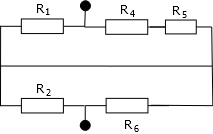
\includegraphics[width=0.5\linewidth]{pr2/2.png}
\end{figure}

\begin{align*}
    R_{45} = R_4 + R_5 &= \SI{180}{\ohm} + \SI{460}{\ohm} = \SI{640}{\ohm}\\
    R_{145} = \frac{R_1 \cdot R_{45}}{R_1 + R_{45}} &= \frac{\SI{250}{\ohm} \cdot \SI{640}{\ohm}}{\SI{250}{\ohm} + \SI{640}{\ohm}} = \SI{179.7752809}{\ohm}\\
    R_{26} = \frac{R_2 \cdot R_6}{R_2 + R_6} &= \frac{\SI{315}{\ohm} \cdot \SI{350}{\ohm}}{\SI{315}{\ohm} + \SI{350}{\ohm}} = \SI{165.7894737}{\ohm}\\
    R_e = R_{145} + R_{26} &= \SI{179.7752809}{\ohm} + \SI{165.7894737}{\ohm} = \SI{345.5647546}{\ohm}\\
\end{align*}

\subsection{Krok 3}
Vypocitame napetie ktore by zdroj U vygeneroval medzi vyznacenymi spojkami. ("H" bude oznacovat hornu spojku a "D" dolnu spojku) 

\begin{align*}
    U_{145} = U_{26} &= U = \SI{180}{\volt}\\
    U_H =  U - U_{145} \cdot \frac{R_1}{R_1 + R_4 + R_5} &= \SI{180}{\volt} - \SI{180}{\volt} 
    \cdot \frac{\SI{250}{\ohm}}{\SI{250}{\ohm} + \SI{180}{\ohm} + \SI{460}{\ohm}} = \SI{129.4382022}{\volt}\\
    U_D =  U_{26} \cdot \frac{R_6}{R_2 + R_6} &= \SI{180}{\volt} \cdot \frac{\SI{350}{\ohm}}{\SI{315}{\ohm} + \SI{350}{\ohm}} = \SI{94.7368421052}{\volt}\\
    U_e = U_H - U_D &= \SI{129.4382022}{\volt} - \SI{94.7368421052}{\volt} =  \SI{34.70136009}{\volt}
\end{align*}

\subsection{Krok 4}
Rezistor $R_3$ teraz pripojime na fiktivny zdroj napatia s $U_e = \SI{34.70136009}{\volt}$ a $R_e = \SI{345.5647546}{\ohm}$

\begin{figure}[!h]
    \centering
    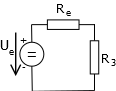
\includegraphics[width=0.2\linewidth]{pr2/3.png}
\end{figure}

\begin{align*}
    U_{R3} = U_e \cdot \frac{R_3}{R_e + R_3} &= \SI{34.70136009}{\volt} \cdot \frac{\SI{615}{\ohm}}{\SI{615}{\ohm} + \SI{345.5647546}{\ohm}} = \SI{22.217488569}{\volt}\\
    I_{R3} = \frac{U_{R3}}{R_3} &= \frac{\SI{22.217488569}{\volt}}{\SI{615}{\ohm}} = \SI{0.0361259976}{\ampere}
\end{align*}